
%%%%%%%%% Latex Template

%Font Size can be changed here
\documentclass[11pt]{article}

\pagestyle{plain}

%%%%%%%%%% EXACT 1in MARGINS %%%%%%%%%%%%
\usepackage[text={6.5in,9in},centering]{geometry}
% %%%%%%%%%%%%%%%%%%%%%%%%%%%%%%%%%%%%

%%%%%%%%%%%%%%%%%%%%%%%%%% DO NOT CHANGE: %%%%%%%%%%%%%%%%%%%%%%%%%%%%%%%%%%%
\renewcommand{\refname}{\begin{center}References Cited\end{center}}
   \setcounter{secnumdepth}{3}
    \setcounter{tocdepth}{2}

\makeatletter

%%\def\section{\@startsection {section}{1}{\z@}{-3.5ex plus -1ex minus -.2ex}{0.1em}{\normalsize\bf}}
\def\section{\@startsection {section}{1}{\z@}{1ex}{0.5em}{\normalsize\bf}}

\def\subsection{\@startsection{subsection}{2}{\z@}{0.5ex}{-1em}{\normalsize\bf}}

\def\subsubsection{\@startsection{subsubsection}{3}{\z@}{0.5ex}{-1em}{\normalsize\bf}}

\def\paragraph{\@startsection{paragraph}{4}{\z@}{0.5ex}{-1em}{\normalsize\bf}}

\def\subparagraph{\@startsection{subparagraph}{4}{\z@}{0.5ex}{-1em}{\normalsize\bf}}

\makeatother
%%%%%%%%%%%%%%%%%%%%%%%%%%%%%%%%%%%%%%%%%%%%%%%%%%%%%%%%%%%%%%%%%%%%%%%%%%%%

% Packages needed
\usepackage[pdftex]{graphicx}
\usepackage{amscd}
\usepackage[pdftex]{color} % black,white,red,green,blue,cyan,magen ta,yellow
\usepackage[pdftex,colorlinks]{hyperref}
\usepackage{amsmath, amsfonts, amssymb,mathrsfs}
\usepackage{multirow}
\usepackage{enumerate}
\usepackage{verbatim}
\usepackage{cite}

\newenvironment{plan}
{\bigskip\hrule\bigskip\centerline{\bf PLAN}\begin{quote}\tt}
{\end{quote}\bigskip\hrule\bigskip}

\newenvironment{instruction}
{\hrule\smallskip
\begin{small}\red\sf\noindent}
{\end{small}
\smallskip\hrule
\bigskip}

\hypersetup{
    bookmarks=true,         % show bookmarks bar?
    unicode=false,          % non-Latin characters in AcrobatÕs bookmarks
    pdftoolbar=true,        % show AcrobatÕs toolbar?
    pdfmenubar=true,        % show AcrobatÕs menu?
    pdffitwindow=true,      % page fit to window when opened
    pdftitle={NSF PIRE 2009},    % title
    pdfauthor={J Xu},     % author
    pdfsubject={Comp Math},   % subject of the document
    pdfnewwindow=true,      % links in new window
    colorlinks=true,       % false: boxed links; true: colored links
    linkcolor=black,          % color of internal links
    citecolor=black,        % color of links to bibliography
    filecolor=black,      % color of file links
    urlcolor=black           % color of external links
}

%%Adler Macros
\usepackage[pdftex]{graphicx}
\def \vec#1{{\bf{#1}}}
\def\pd#1#2{\frac{\partial #1}{\partial #2}}
\def \mat#1{\underline{\underline{#1}}}
\def \mylim#1#2{\lim_{#1 \rightarrow #2}}
\newcommand{\bi}{\begin{itemize}}
\newcommand{\ei}{\end{itemize}}
\newcommand{\func}{\mathcal{F}}
\newcommand{\vw}{\mbox{\boldmath$\omega$}}
\newcommand{\vb}{\mbox{\boldmath$\beta$}}
\newtheorem{thm}{Theorem}
\newtheorem{cor}[thm]{Corollary}
\newtheorem{lem}[thm]{Lemma}
\newcommand{\mV}{\mathcal{V}}
\newcommand{\mL}{\mathcal{L}}

\newenvironment{jhalist}{
\vspace*{-6pt}
\begin{list}{\labelitemi}{\leftmargin=1.4em}
 \setlength{\itemsep}{1pt}
 \setlength{\parskip}{0pt}
 \setlength{\parsep}{0pt}
}{\end{list}}


\begin{document}


%%%%%%%%% PROPOSAL -- 2 pages

\setcounter{section}{0}

\begin{center}
\textbf{Numerical Analysis on Black-Scholes Model: An FEM Method}\\
\author{}{Sheng Xu}\end{center}
\section{Introduction}

The Black-Scholes Model is a mathematical model of financial market containing derivative investment instruments. From the model, we can find a theoretical estimate of the price of European Options. The formula is called the "Black-Scholes Formula". Many empirical tests have shown that the Black�CScholes price is "fairly close" to the observed prices, although there are well-known discrepancies such as the "option smile".
\\

Currently, many numerical methods in Partial Differential Equations, such as simulation-based methods, the lattice methods, have been well applied to the "Black-Scholes Formula", delaying the study of other numerical methods like finite elements methods, which has been widely used in many fields of science and engineering.
\\

\section{Goal of this poject}
In this project, we will adapt the FEM methods into the "Black-Scholes Formula":
\\
\begin{align*}
\frac{\partial V}{\partial t}+rS \frac{\partial V}{\partial S}+\frac{1}{2} \sigma ^2 S^2 \frac{\partial ^2 V}{\partial S ^2}-rV=0...[1]
\end{align*}
\\
where S is a real asset value, $0 \leq S \leq \infty$, V is the (real) option price, r is the risk-free rate, t is the time since the option was
issued, $0 \leq t \leq T$ , and �� is the real asset volatility. Eq. (1) is a backward moving equation, i.e. it is solved from
the future to the present time.\\
For an European call option the time condition becomes a final condition because its value is known at the maturity date
t = T and it is defined as its intrinsic value by:
\begin{align*}
V(S, T ) = max(S - K, 0), \forall S.
\end{align*} 

\vspace{2pt}
We will explore the way to discrete the variables and assemble the matrix to solve for the solution and compare the solution the theoretical results of options. Meanwhile, we also want to choose the boundary condition for the equation. The study is mainly focused on European Options. If time permitted, we might also study the formula of American Options.\\
\begin{center}
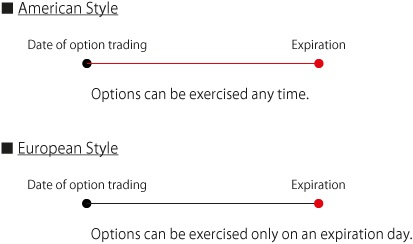
\includegraphics [width = .8\textwidth]{US_EU_DIFF1.jpg}
\\
Figure 1: Time to exercise\\

\vspace{20pt}

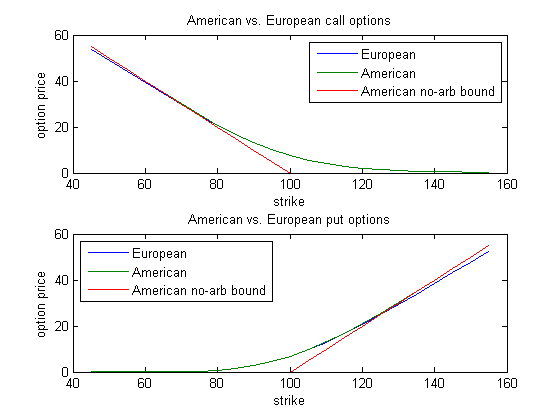
\includegraphics [width = .8\textwidth]{US_EU_DIFF2.jpg}\\
Figure 2: Different Value at Strikes\\
\end{center}

\clearpage
\section{Reference}
[1] Andalaft-Chacur A, Ali M M, Salazar J G. Real options pricing by the finite element method[J]. Computers and Mathematics with Applications, 2011, 61(9): 2863-2873.\\

[2] F. Black, M. Scholes, The pricing of options and corporate liabilities, The Journal of Political Economy 81 (1973) 637�C654. \\

[3] Golbabai A, Ballestra L V, Ahmadian D. Superconvergence of the finite element solutions of the Black�CScholes equation[J]. Finance Research Letters, 2013, 10(1): 17-26.\\

[4] C. Zhang, Pricing American options by adaptive finite element method, Mathematics Department University of Maryland, 2005\\



\end{document}


